\subsection{Ellipsoids in added variable plots}
In contrast to the marginal, bivariate views of the relations of several predictors to a
response (e.g., such as shown in the top row of \figref{fig:vis-reg-coffee11}), added-variable plots
(aka partial regression residual plots) show the partial relations between the response and
each predictor, where the effects of all other predictors have been controlled or adjusted for.

\begin{figure}[htb]
 \begin{minipage}[b]{.49\linewidth}
  \centering
  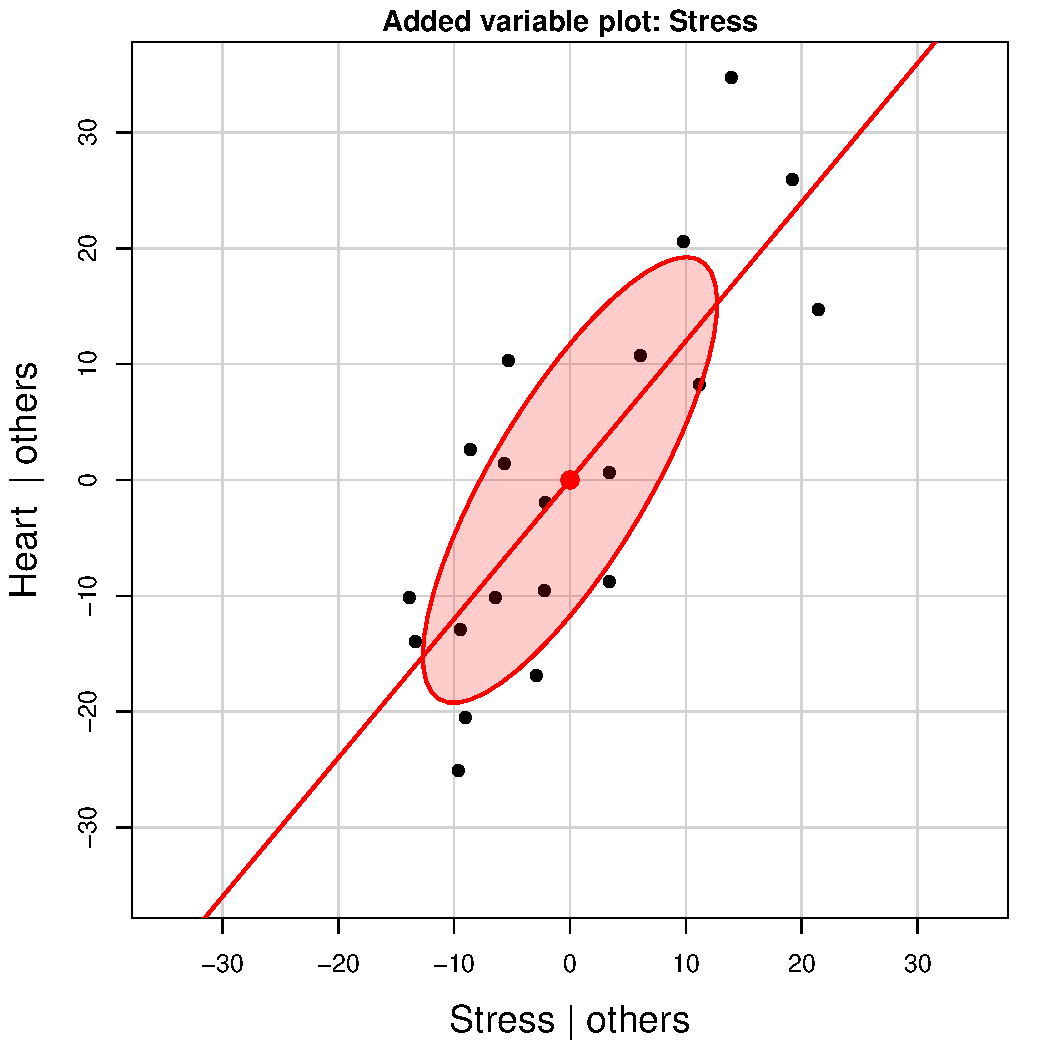
\includegraphics[width=1\linewidth]{fig/coffee-avplot1}
%  \caption{}%
%  \label{fig:}
 \end{minipage}%
 \hfill
 \begin{minipage}[b]{.49\linewidth}
  \centering
  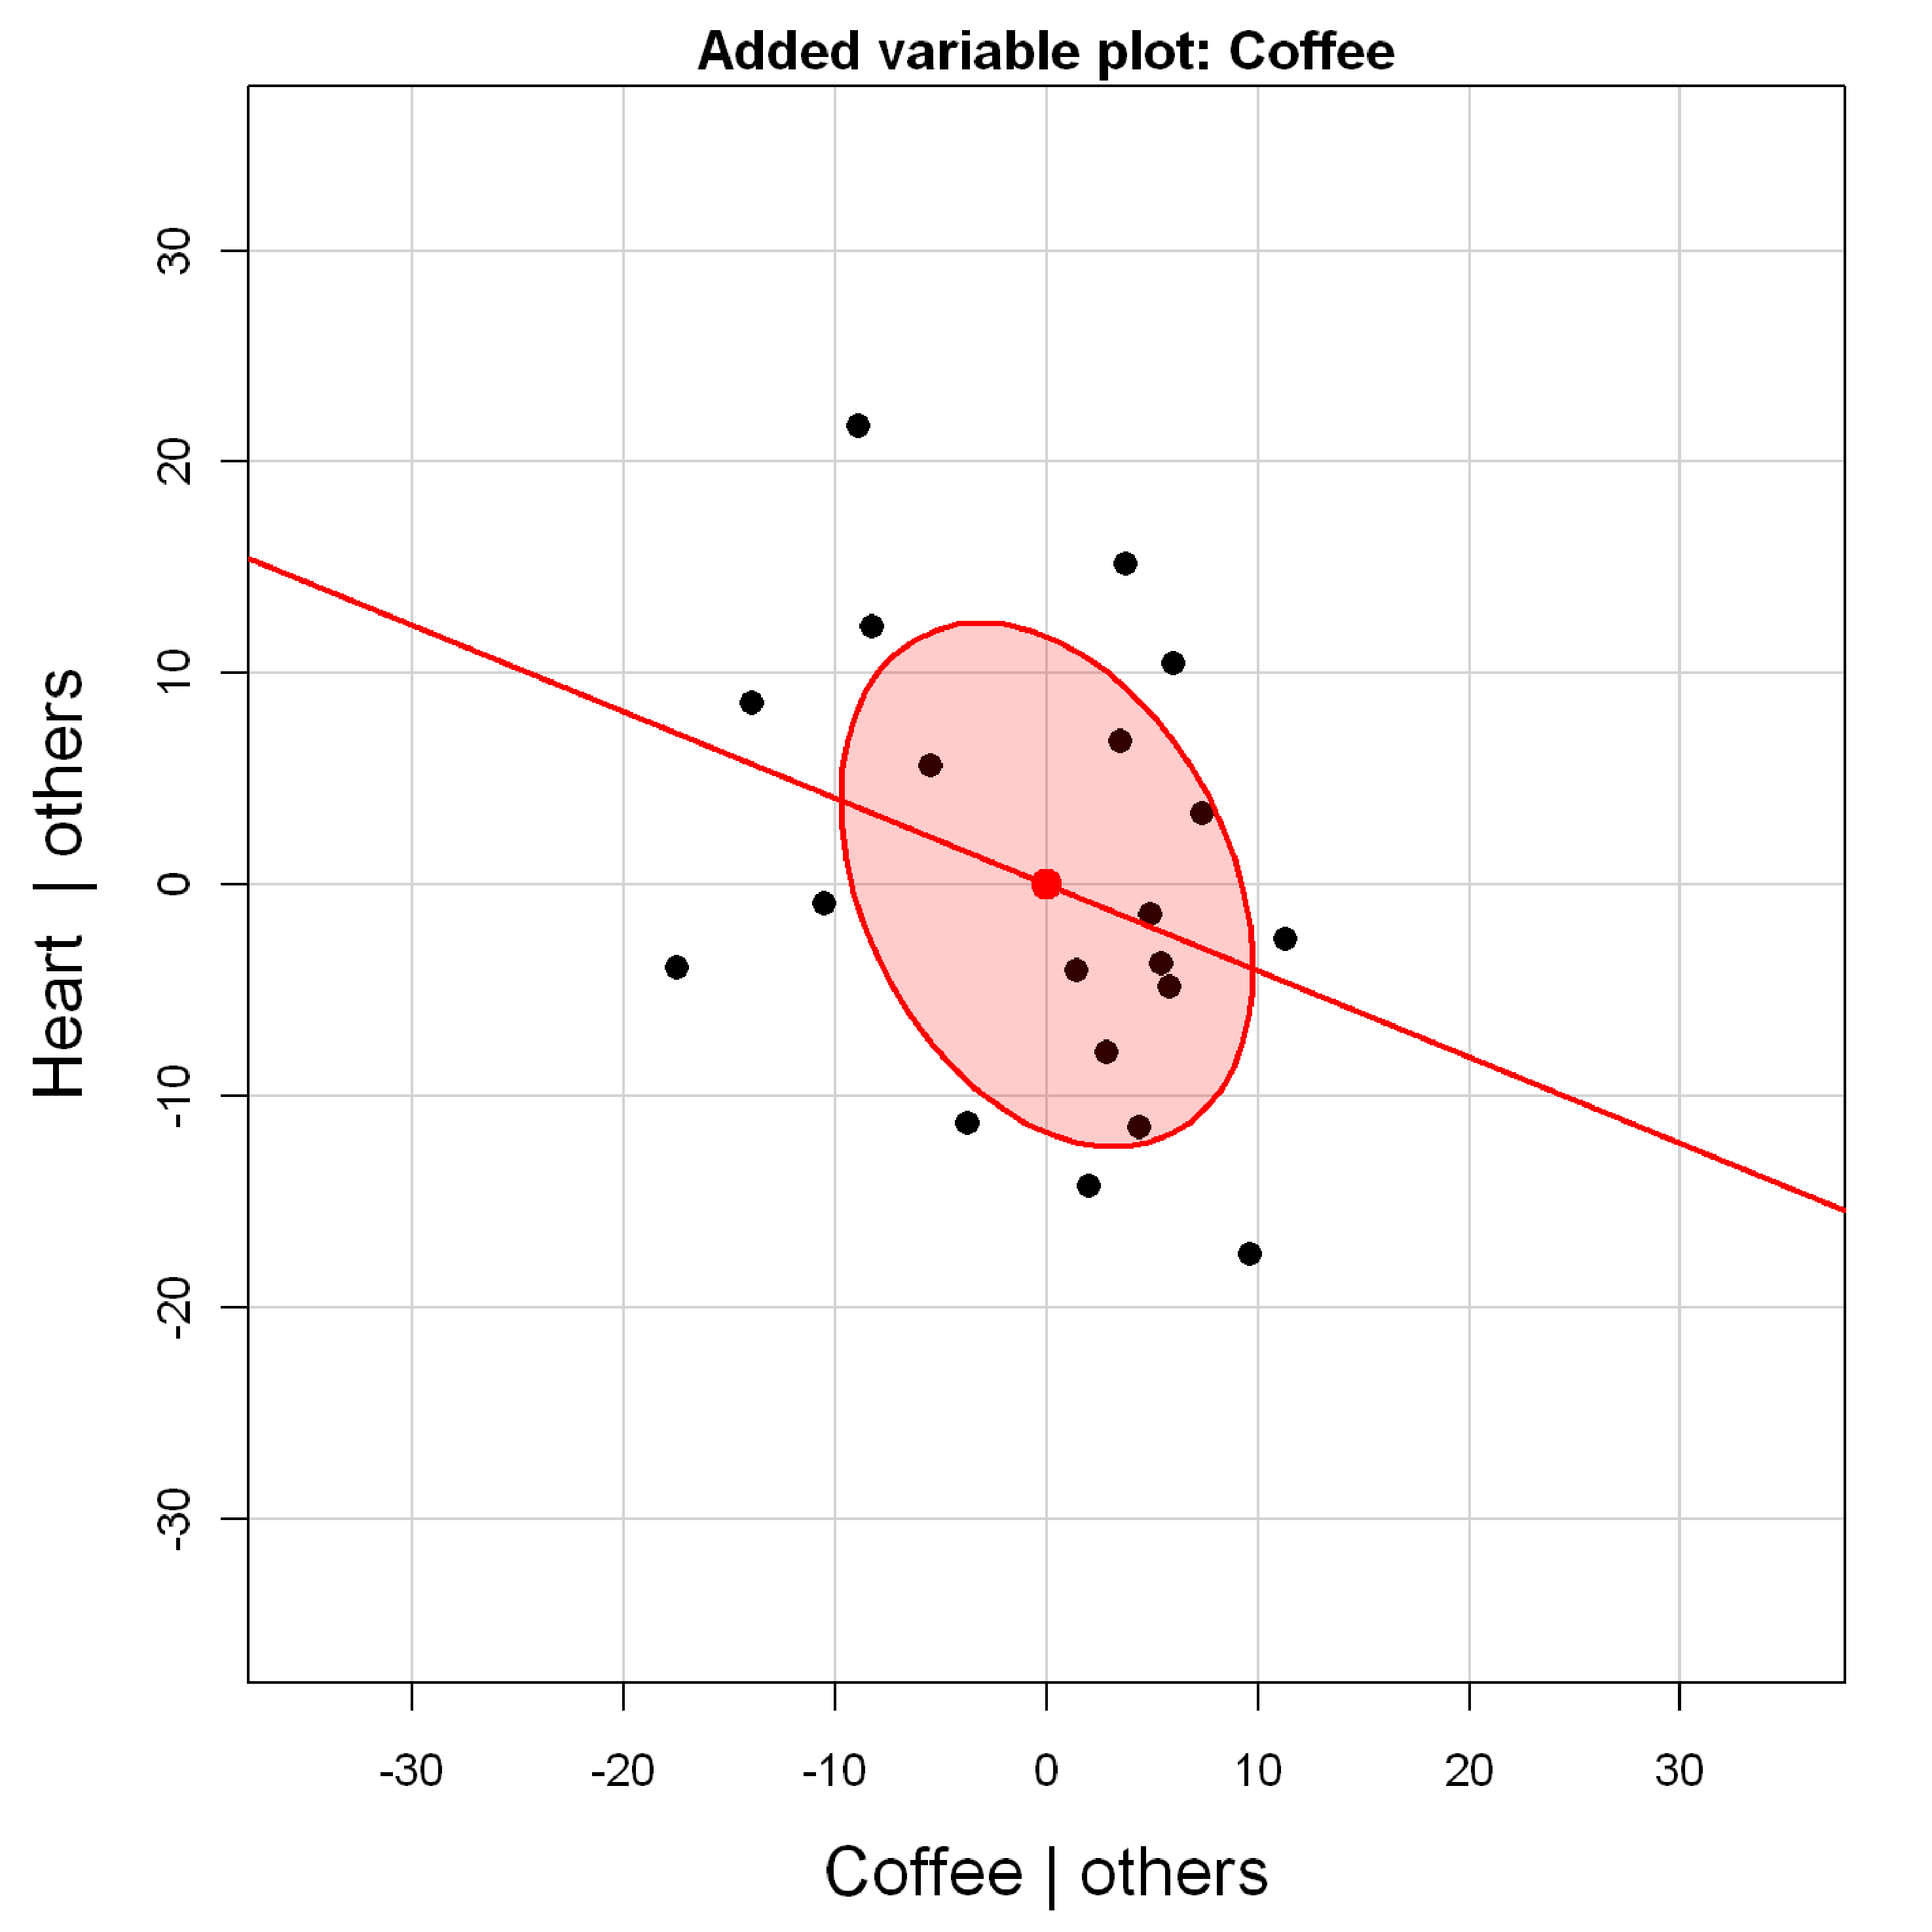
\includegraphics[width=1\linewidth]{fig/coffee-avplot2}
 \end{minipage}
  \caption{Added variable plots for Stress and Coffee in the multiple regression predicting Heart disease.
Each panel shows the 50\% conditional data ellipse for partial residuals (shaded, red) as well as the marginal 50\% 
data ellipse for the $(x, y)$ variables, shifted to the origin.
Arrows connect the mean-centered marginal points (open circles) to the partial residual points (filled circles).}
  \label{fig:coffee-avplot}
\end{figure}
